\documentclass[letterpaper,11pt]{article}
\usepackage{tabularx} % extra features for tabular environment
%\usepackage{amsmath}  % improve math presentation
\usepackage{graphicx} % takes care of graphic including machinery
\usepackage[margin=1in,letterpaper]{geometry} % decreases margins
%\usepackage{cite} % takes care of citations
\usepackage[final]{hyperref} % adds hyper links inside the generated pdf file
\hypersetup{
	colorlinks=true,       % false: boxed links; true: colored links
	linkcolor=blue,        % color of internal links
	citecolor=blue,        % color of links to bibliography
	filecolor=magenta,     % color of file links
	urlcolor=blue         
}
\usepackage{biblatex}
\addbibresource{bibItem.bib}
\usepackage{blindtext}
%++++++++++++++++++++++++++++++++++++++++


\begin{document}

\begin{center}
{\Large Frankenstein: Advanced Wireless Fuzzing to Exploit New Bluetooth Escalation Targets} 

{Jan Ruge and Jiska Classen, Secure Mobile Networking Lab, TU Darmstadt;
Francesco Gringoli, Dept. of Information Engineering, University of Brescia;
Matthias Hollick, Secure Mobile Networking Lab, TU Darmstadt}
\bigskip

{\large Writer: Akib Jawad Nafis}
\date{\today}
\end{center}


%\section{Summary}
%
%Your summary goes here 
%
%%\blindtext %delete this line
%
%
%\section{Strengths and Weaknesses}
%
%3-Key points for strengths and weaknesses each.
%
%%\blindtext % delete this line

\section{Introduction}

Radio frequency protocols or implementations have always been a huge target for attackers. The reason behind this would be a huge attack surface. An attacker can attack wireless protocols even before it is connected to the network. Most of the wireless protocol implementation is closed source. As a result fuzzing became the best way to find bugs in these implementations. Protocol fuzzing over the air is pretty slow. We have to depend on the wireless transmission time. At the same time there can be interference while fuzzing over the air. Dependency on physical devices, limitation while repeating an experiment, complexity in debugging also contributes to the issues of over the air fuzzing. Making the wireless fuzzing faster at the same time less clunky is a great research problem. 
\subsection{Wireless Fuzzing of Bluetooth}
One of the most widely used RF protocol implementation would be Bluetooth. Almost all of the smartphones and portable computers today has a Bluetooth chip in it. At the same time security of Bluetooth has always been kind of questionable. Bluetooth stack is divided on two parts. Host (Operating System of the device holding that Bluetooth chip) and Bluetooth Controller chip. These two in connected with a layer named HCI (Host Controller Interface). Software in the Bluetooth controller chip is called firmware. Firmware of a Bluetooth chip or any wireless chip is closed source. Hence it is hard to debug but vulnerabilities residing in the firmware can be catastrophic. At the same time fixing those vulnerabilities after deployment is another huge problem. Because firmware resides in ROM chip of the hardware, not easy to update. Fix have to come the chip vendor itself. Some vulnerability in the firmware can be remain hidden even from the operating system. As some portion of the Bluetooth hardware doesn't require any kind of interaction with the host stack. So fuzzing the Bluetooth firmware to find out bugs before an attacker choose to exploit them is a great idea. Combining these with the idea to improve over the air fuzzing is our goal in this project. We choose broadcom Bluetooth firmware to fuzz as it is widely used.

\subsection{Prior Work}
Fuzzing Bluetooth protocol has been mostly limited to fuzzing the host stack. Bluetooth Firmware has not been fuzzed public prior to this work. Prior to this Bluetooth Firmware research was mostly about extending the capability of the chip. There were research about security of the Bluetooth Firmware but it was manual analysis. btlejack \cite{btlejack} extends capability of the BLE at the same describing man in the middle attack. InternalBlue \cite{DBLP:journals/corr/abs-1905-00631} used reverse engineering of Bluetooth Firmware to read/manipulate low layer frames. It also discovers a bug in the Broadcom chip.
Over the air fuzzing has been done in deepsec \cite{deepsec} but it focuses on host part of the Bluetooth stack. Other fuzzing efforts was based on drivers and operating systems. Syzkaller\cite{syzkaller} supports fuzzing HCI in linux. Apart from broadcom chip, Marvel Avastar\cite{marvel-avastar} WiFi chip was fuzzed using afl-unicorn\cite{afl-unicorn}. TriforceAFL\cite{TriforceAFL} uses similar QEMU based fuzzing but it modify the QEMU itself for other supports. On the other hand Frankenstein here uses QEMU as a userspace program for support it uses hooking the firmware. LTEFuzz \cite{8835363} fuzzes LTE network over the air and found vulnerabilities in core network components.  


\section{Approaches Taken}
To solve problems of the over the air fuzzing authors took a new approach. It is emulating the firmware to create a virtual chip. By emulation authors reduce latency from host to chip communication. They didn't have to depend on another chip to send packets over the air. They were able to cut down the transmission time by generating packets in the device itself. Emulated virtual chip can be connected to the Bluetooth host side of linux system. Thus creating a full system emulation environment. 
\begin{figure}[htp]
    \centering
    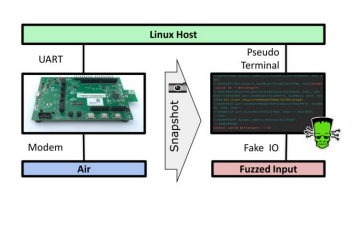
\includegraphics{images/No-Poc-No-Fix-.png}
    \caption{Emulation Based Fuzzing}
    \label{fig:Emulation Based Fuzzing}
\end{figure}
\subsection{Emulating the firmware}
Authors pulled snapshot from the physical device and then used it as a firmware to emulate in QEMU. But a snapshot can't be directly emulated. It is just a binary. A elf executable file must be generated to execute it in the QEMU environment. That elf executable need some more support. 

This frankenstein will run as a user-space program it doesn't support any interrupt or timer itself. But Bluetooth firmware has it's own interrupt and timer handlers. These interrupt and timer handlers need to be implemented manually for the virtual chip. It could have been done in the QEMU itself, but then that QEMU emulation will not be user-mode emulation. Along with this support debug symbols and coverage hooks must be included in the firmware for fuzzing. Including all of those a virtual chip is generated. 

\subsection{Connecting Virtual Chip to the Host}
To connect this virtual chip to the linux host Pseudo Terminal is used. Pseudo terminal is basically a pipe to connect two programs. Master end of the pipe belongs to the virtual chip and slave end of the pipe belongs to the host side of Bluetooth stack.
\subsection{Random packet generation} 
To generate inputs packets for the firmware a virtual modem is created. Virtual modem creates various types of packet to trigger various portion of the firmware codebase.
\subsection{Mutating inputs while generating inputs} 
Frankenstein uses a different type of mutation techniques. Typical fuzzers uses input as a large binary object and modify it. Frankenstein modified this process slightly. Instead of considering whole packet as a binary object, it took two parts of the packet (Sequence No and Data) and modified them separately. 
This method results in better code coverage[\ref{fig:Code coverage}].
\begin{figure}[htp]
    \centering
    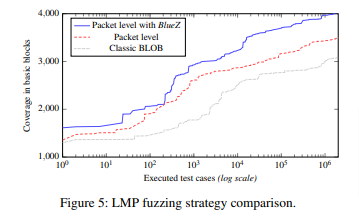
\includegraphics{images/code-coverage.png}
    \caption{Code coverage}
    \label{fig:Code coverage}
\end{figure}
Classic blob (grey line) represents mutation of the packet as a binary blob. Packet Level (red line) is modification to packet data only. Packet Level with BlueZ includes mutation of both sequence no and packet data.
\subsection{Evaluation based of bugs found} 
Frankenstein discovered two types of bug in the Bluetooth firmware. One is Remote Code Execution based and another is heap corruption based. Types of Bugs and their CVEs are included in the list below. 
\begin{table}[h]
    \centering
    \begin{tabular}{|p{65mm}|p{65mm}|}
    \hline
    RCE bugs & Heap Corruption Bugs \\
    \hline
     Link Key Extraction. &  Device Scanning EIR (CVE-2019-11516).  \\
     \hline
    Disabling Wifi by writing a specified value while testing in a wifi/bluetooth combo chip. (CVE-2019-15063). &  Any BLE Packet (CVE-2019-13916). \\
    \hline
     &  Any ACL Packet (CVE-2019-18614). \\
    \hline
     &  BlueFrag (CVE-2020-0022).\\
    \hline
    \end{tabular}
    \caption{Vulnerabilities and CVE's found by frankenstein}
    \label{tab:lseek()_table}
\end{table}
\subsection{Evaluation based on novelty and speed} 
Since it is the first systemic approach to find bugs in the bluetooth firmware via emulation based fuzzing, it has novelty in it. Also it increases efficiency than over the air fuzzing.

\section{Deliverable}
\label{sec:deliverable}
Two types deliverable while reproducing this work. 
\begin{itemize}
    \item Reproducing their emulations.
    \item Reproducing CVE using the emulator.
\end{itemize}
\subsection{Reproducing their emulations} 
Systemwise build will generate 8 emulations. 
\begin{figure}[htp]
    \centering
    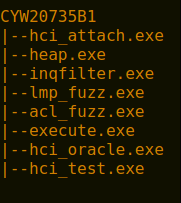
\includegraphics{images/building-sourcde-code.png}
    \caption{emulations}
    \label{fig:emulations}
\end{figure}
Emulating all modules will be time consuming. I'll try to emulate and report my finding form the execute.exe, heap.exe, hci\_attach.exe, inqfilter.exe, lmp\_fuzz.exe, acl\_fuzz.exe. [It might change since I don't know which emulation takes how much time]  
\subsection{Reproducting CVEs}
I will reproduce two CVEs. 
\begin{itemize}
    \item Device Scanning EIR (CVE-2019-11516)
    \item Any BLE Packet (CVE-2019-13916)
\end{itemize}
I won't be able to to reproduce some of the CVE's due to device constraint. 
\begin{itemize}
    \item Any ACL Packet (CVE-2019-18614) [Reproducing this experiement bricked a module of authors. Also lack of time :( ] 
    \item BlueFrag (CVE-2020-0022). [Need an Android 8.0-9.0 device wth this specific bluetooth chip to follow the steps.]
    \item Disabling Wifi by writing a specified value while testing in a wifi/bluetooth combo chip. (CVE-2019-15063) [It's done on wifi/bluetooth combo chip. I don't have any neither physical nor virtual.]
\end{itemize}

% \section{Timeline}
% I'll have 6 week time before I submit this work. I'll try to follow this timeline. Timeline is subject to be variable with the complexity of the project or obstacle.

% \begin{table}[h]
%     \centering
%     \begin{tabular}{|p{10mm}|p{80mm}|}
%     \hline
%     Week 1 & Mapping concepts form papers to codebase. \\
%     \hline
%     Week 2 & Emulation without host and with host attached (execute.exe, hci\_attach.exe, lmp\_fuzz.exe) \\
%     \hline
%     Week 3 &  Try to emulate and explain acl\_fuzz.exe, inqfilter.exe. \\
%     \hline
%     Week 4 &  Reproducing Extended Inqiry Respose heap corruption (CVE-2019-11516). Reproducing Low Energy Reception Heap Overflow (CVE-2019-13916).\\
%     \hline
%     Week 5 &  Presentation\\
%     \hline
%     Week 6 &  Project Report\\
%     \hline
%     \end{tabular}
%     \caption{Vulnerabilities and CVE's found by frankenstein}
%     \label{tab:lseek()_table}
% \end{table}
\section{Experiments}
As per proposal I emulated 5 of the 8 emulations mentioned in the project. Also reproduced two CVEs from this project. Initially I'll describe experimental setup. Then I'll go through the emulations. Later I'll describe how CVE's are reproduced and what triggered those bugs.
\subsection{Experimental Setup}
Authors goal was to execute Bluetooth firmware in a virtual environment so that they can fuzz the firmware easily. To do this, authors copied all the memory segments of a running firmware. Authors copied the memory segment with a script. Authors provided memory segments of the firmware CYW20735 Bluetooth evaluation board. Patched the firmware to execute it without the actual hardware. A hooking mechanism which mainly use c-construct is used for patching process. Then run the virtual firmware to test various portion of the firmware. To check various portion of the firmware authors created multiple emulations which will execute in the virtual environment.
\subsection{Emulation: execute.exe}
In this emulation authors simply confirmed they can interact with virtual firmware executing in QEMU. They also confirmed firmware is executing it's three threads(bttransport, lm and idle) correctly. When both bttransport and lm thread is waiting for events firmware will moe to idle thread. When firmware reaches that idle thread authors hooked their external code to check that they can interact with the firmware. From the emulation \ref{fig:execute.exe} we can see firmwre thread switching and once it reaches idle state as per external code it exits execution.
\begin{figure}[!h]
    \centering
    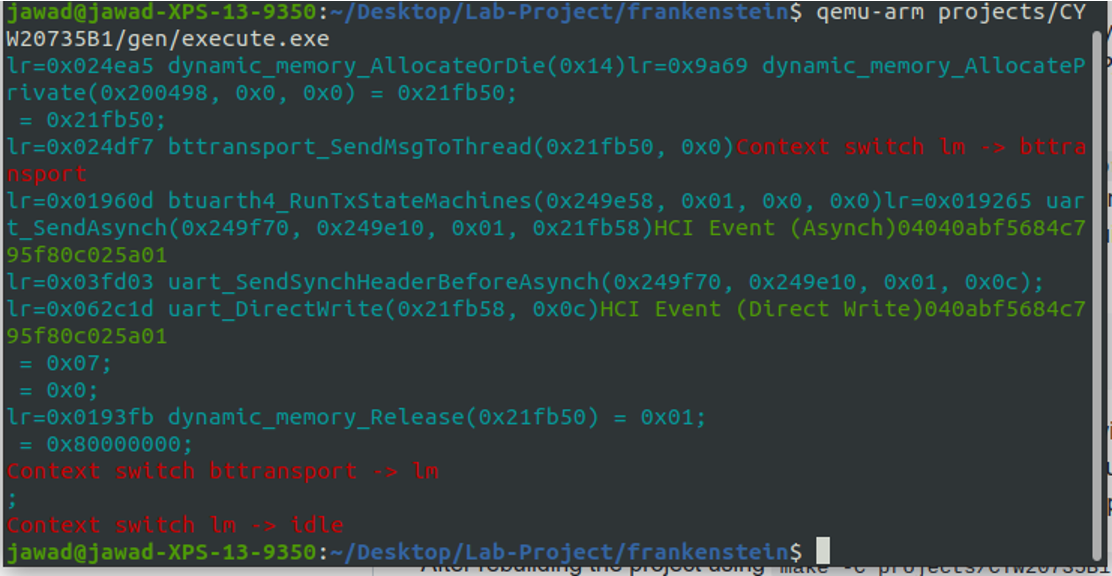
\includegraphics[width=\textwidth]{images/execute.png}
    \caption{Emulating execute.exe}
    \label{fig:execute.exe}
\end{figure}
\subsection{Emulation: hci\_attach.exe} 
In this emulation author confirmed that the firmware can be executed with the Bluetooth stack of operating system. They used linux bluetooth stack Bluez to connect the firmware. After successful connection it will act as a complete virtual Bluetooth device. To check functionality of the virtual bluetooth device, I tried scanning for bluetooth devices\ref{fig:hci_attach.exe}. Random packets(containing bluetooth device addresses) are feed to the virtual device via terminal. 
\begin{figure}[!h]
    \centering
    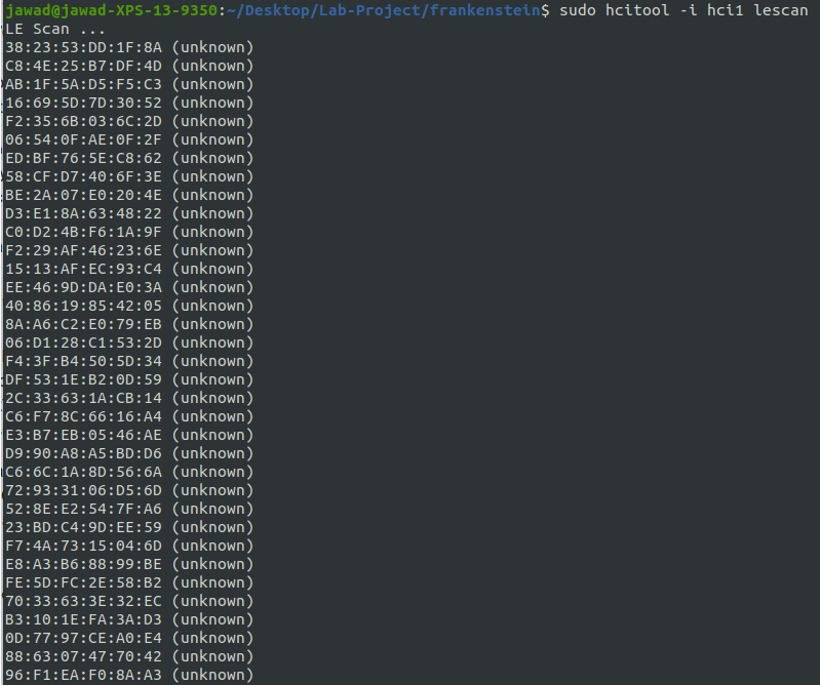
\includegraphics[width=\textwidth]{images/scanning_devices.png}
    \caption{Emulating hci\_attach.exe}
    \label{fig:hci_attach.exe}
\end{figure}
\subsection{Emulation: lmp\_fuzz.exe} 
In this emulation, authors executed link management protocol implementation of the firmware. Random packets are feed to the firmware by hooking a function of the firmware \verb|lm_LmpReceived()|. In a real device this function is called when a new link management packet has been received. Fuzzing this experiment didn't trigger any bug. Figure \ref{lmp.exe} shows the relevant function calls while processing random link management packets. This experiment also emulated the portion when a lmp packet creates a hci event at host end. Generated hci command is sent to the host by using \verb|lm_sendCmd()| function. 
\begin{figure}[!h]
    \centering
    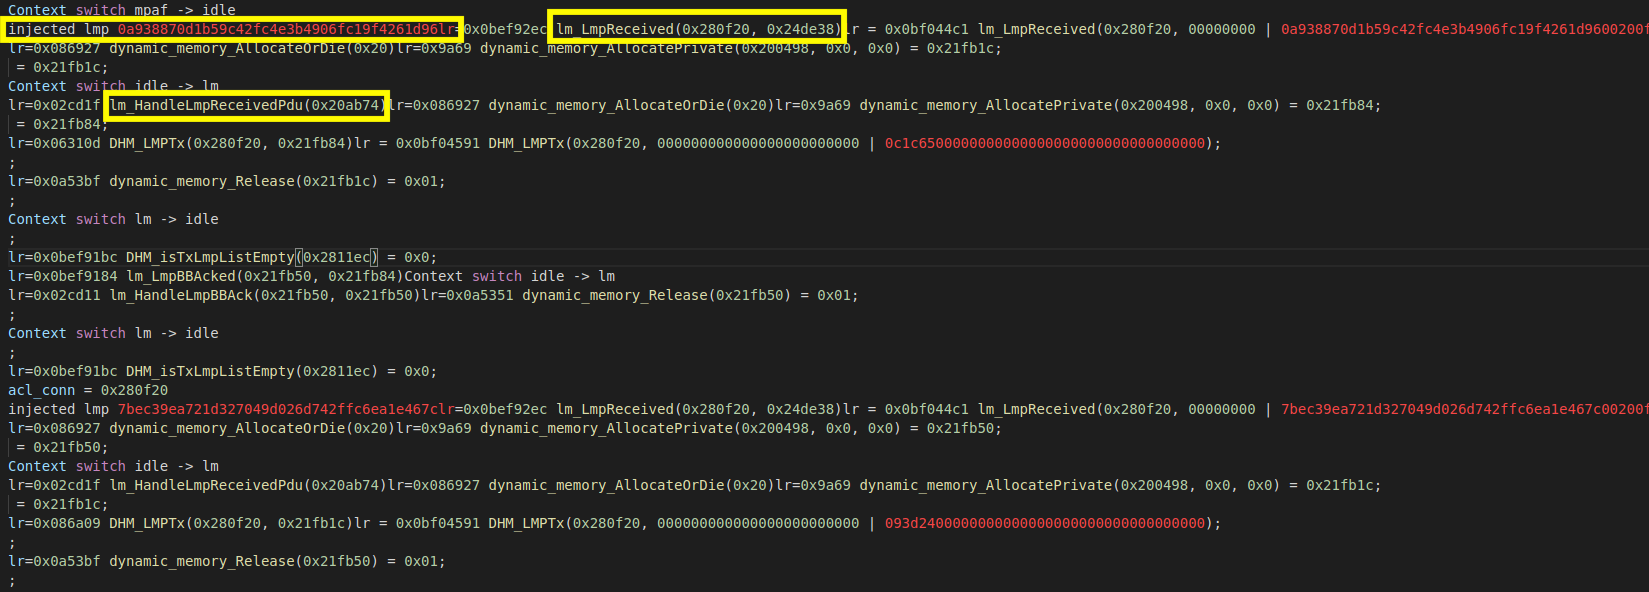
\includegraphics[width=\textwidth]{images/injected_lmp.png}
    \caption{Emulating lmp\_fuzz.exe}
    \label{fig:lmp.exe}
\end{figure}
\subsection{Emulation: acl\_fuzz.exe} 
Similar to link management protocol fuzzing, authors fuzzed asynchronous connection-less packet transfer process. Authors feed the system random payload packet to observe the packet sending and receiving process. Fuzzing this experiment didn't trigger any bug neither in authors experiment nor in my experiment. Goal was to check firmware is executing correctly in the virtual environment. Figure \ref{fig:aclSending} and \ref{fig:aclReceiving} shows the relevant function calls while processing random acl packets. 
\begin{figure}
    \centering
    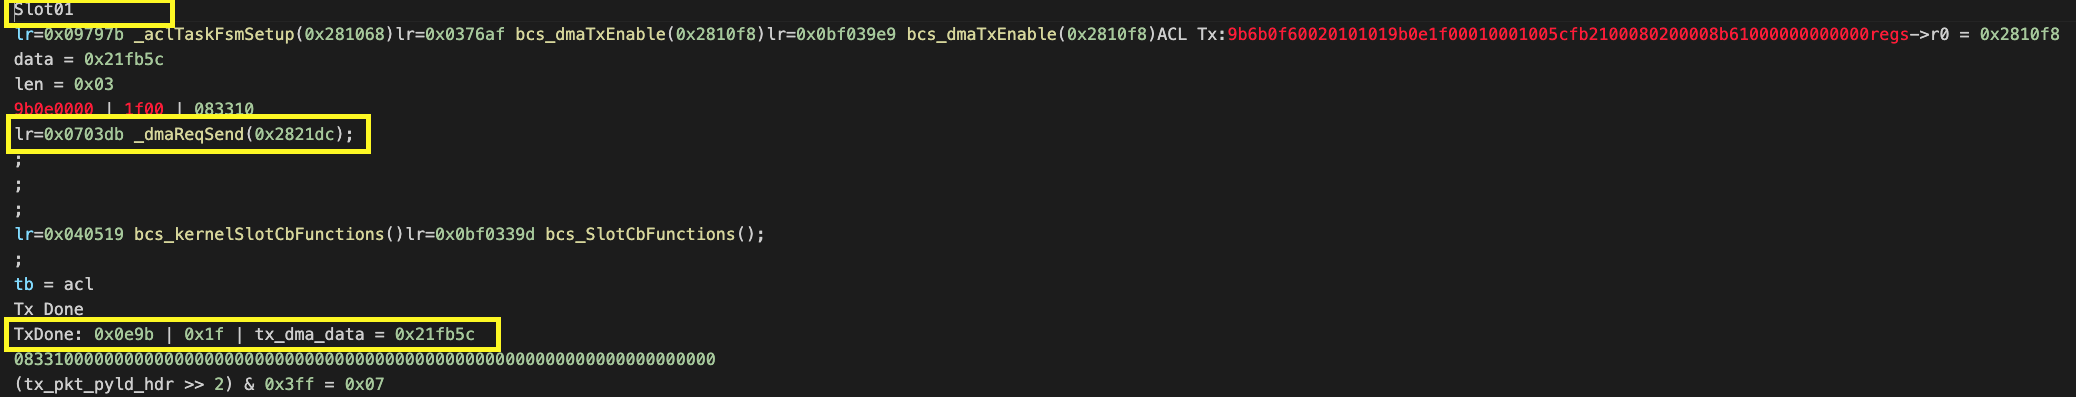
\includegraphics[width=\textwidth]{images/acl_Send_data.png}      \caption{ACL packet sending}
    \label{fig:aclSending}
\end{figure}
\begin{figure}
    \centering
    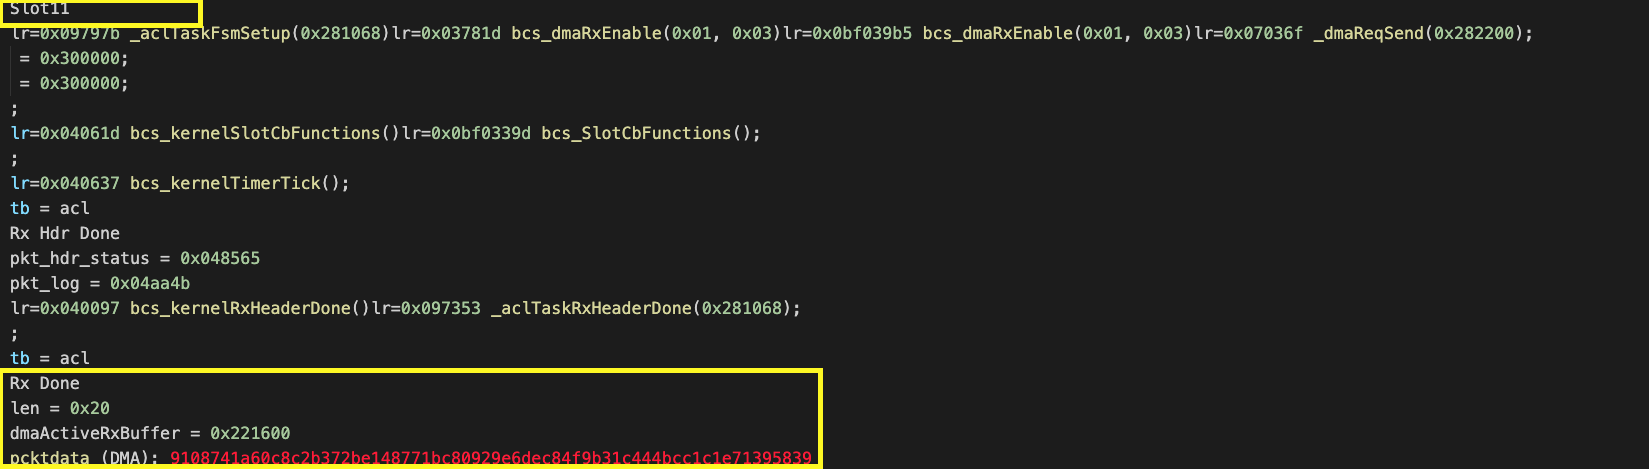
\includegraphics[width=\textwidth]{images/acl_receive_data.png}      \caption{ACL packet receiving}
    \label{fig:aclReceiving}
\end{figure}

\subsection{Reproducing CVE-2019-11516}
It is a bug which causes the firmware to crash while searching for other bluetooth devices nearby. When a bluetooth device is scanning for other devices, it sends a packet. This packet is called inquiry packet. When nearby bluetooth devices wants to respond to this inquiry they can send a response packet. In some cases, these nearby bluetooth devices sends an extended inquiry response. Problem is a malformed extended inquiry response will crash the inquiring firmware. Here malformed response means RFU bits of the inquiry response are anything but 0. 

In my experiment, I tried to scan for devices with the virtual bluetooth device. While fuzzer is feeding the virtual bluetooth device with random inquiry responses. After sometimes firmware of the device which was scanning crashed. Because a inquiry response had the RFU bits set. And while processing the response in the function \verb|inqfilter_registerBdAddr()| firmware crashed. Figure \ref{fig:inqfilter_cve} shows the experiment where in the right terminal virtual device is scanning and the left terminal shows what is happening inside the firmware.
\begin{figure}
    \centering
    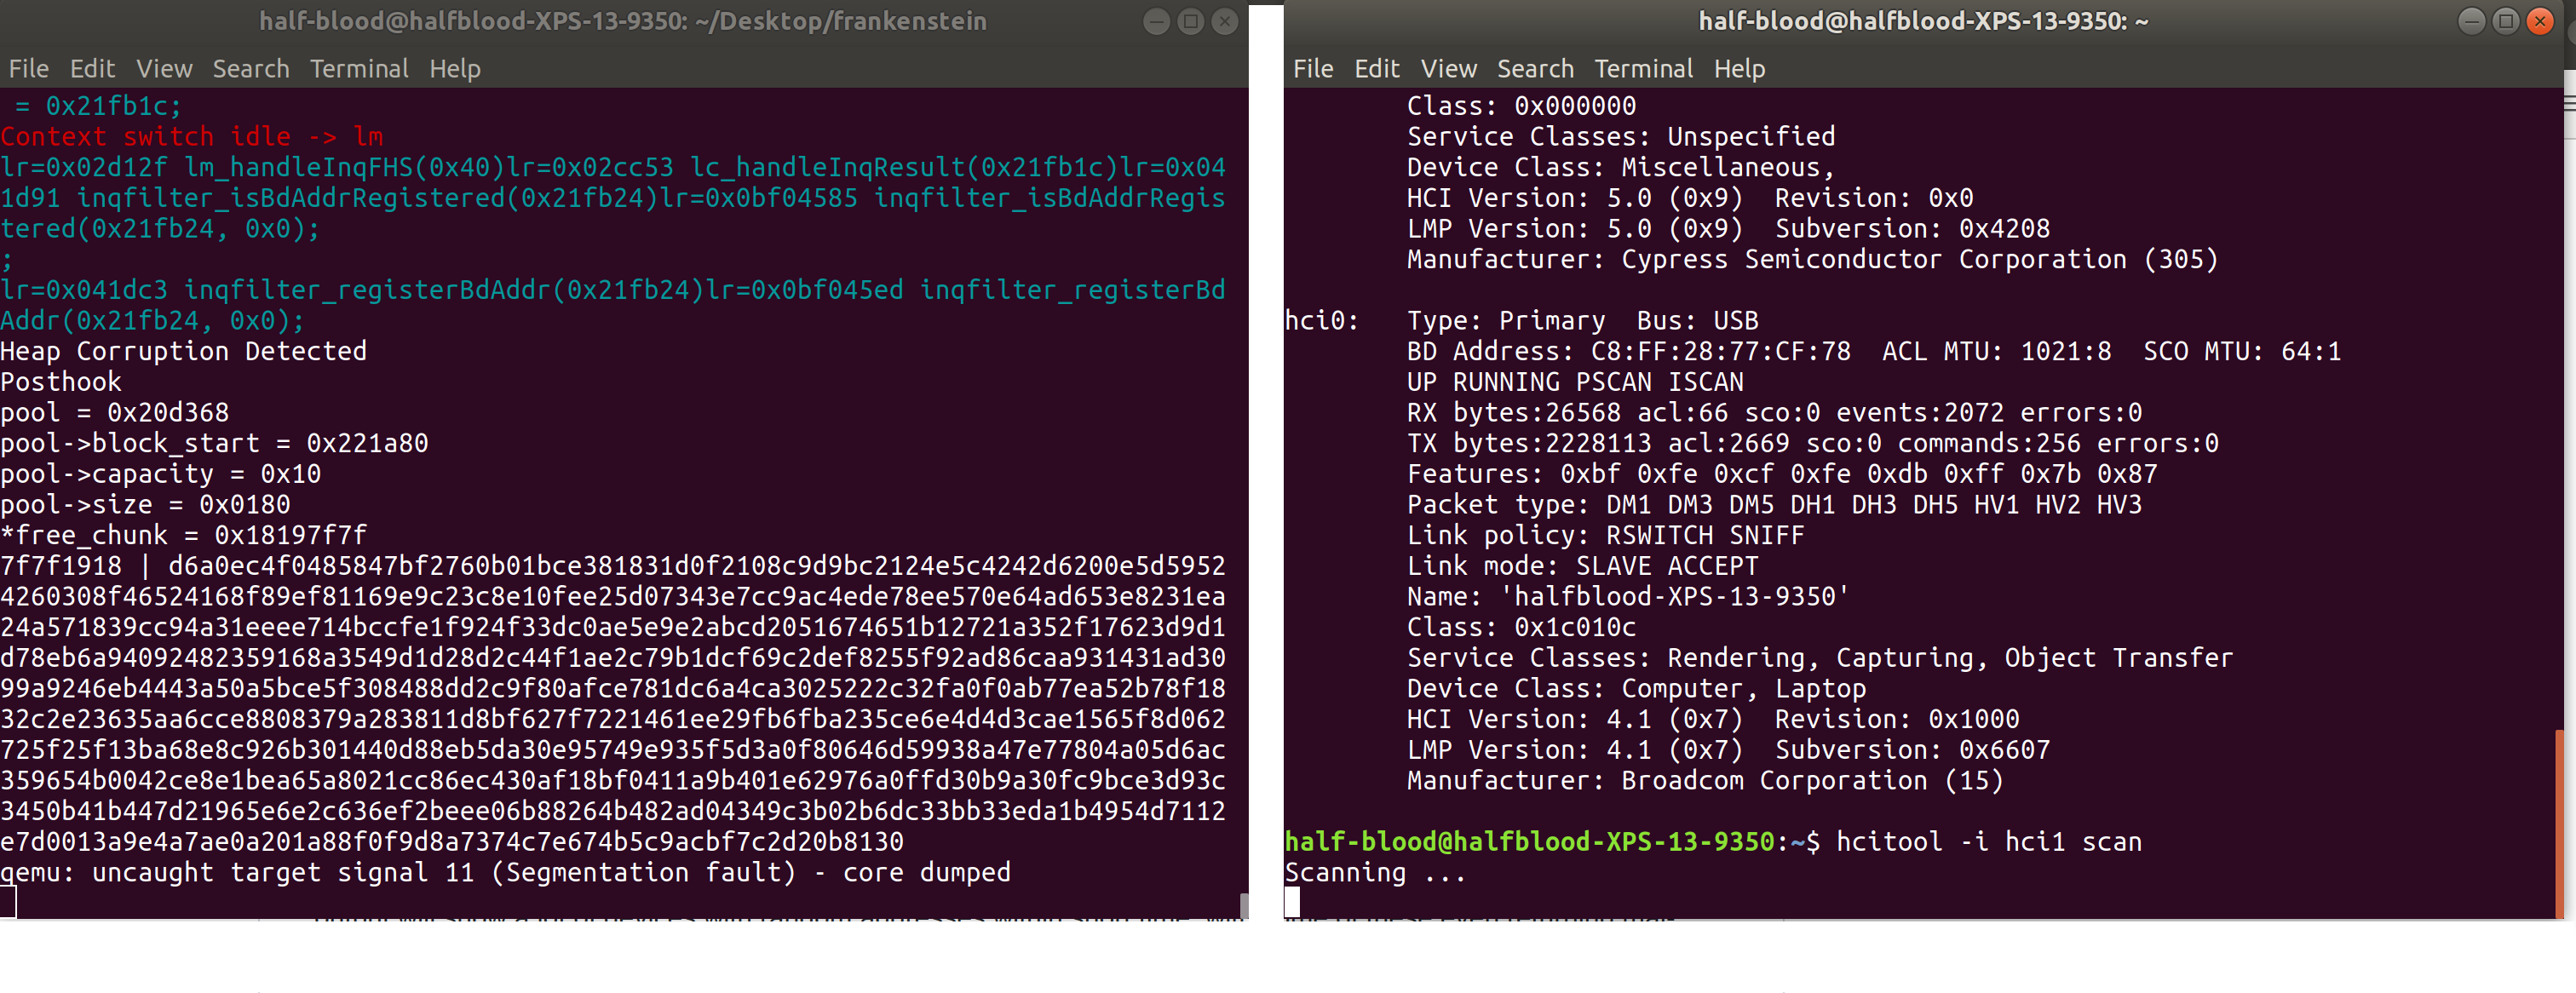
\includegraphics[width=\textwidth]{images/first-cve.png}      \caption{Reproducing CVE-2019-11516}
    \label{fig:inqfilter_cve}
\end{figure}

\subsection{Emulation: inqfilter.exe}
This emulation is created to show the bug mentioned in the previous section. In this emulation authors simply calls the function \verb|inqfilter\_registerBdAddr()| with a crafted inquiry response. Results are shown in the figure \ref{fig:inqfilter}
\begin{figure}
    \centering
    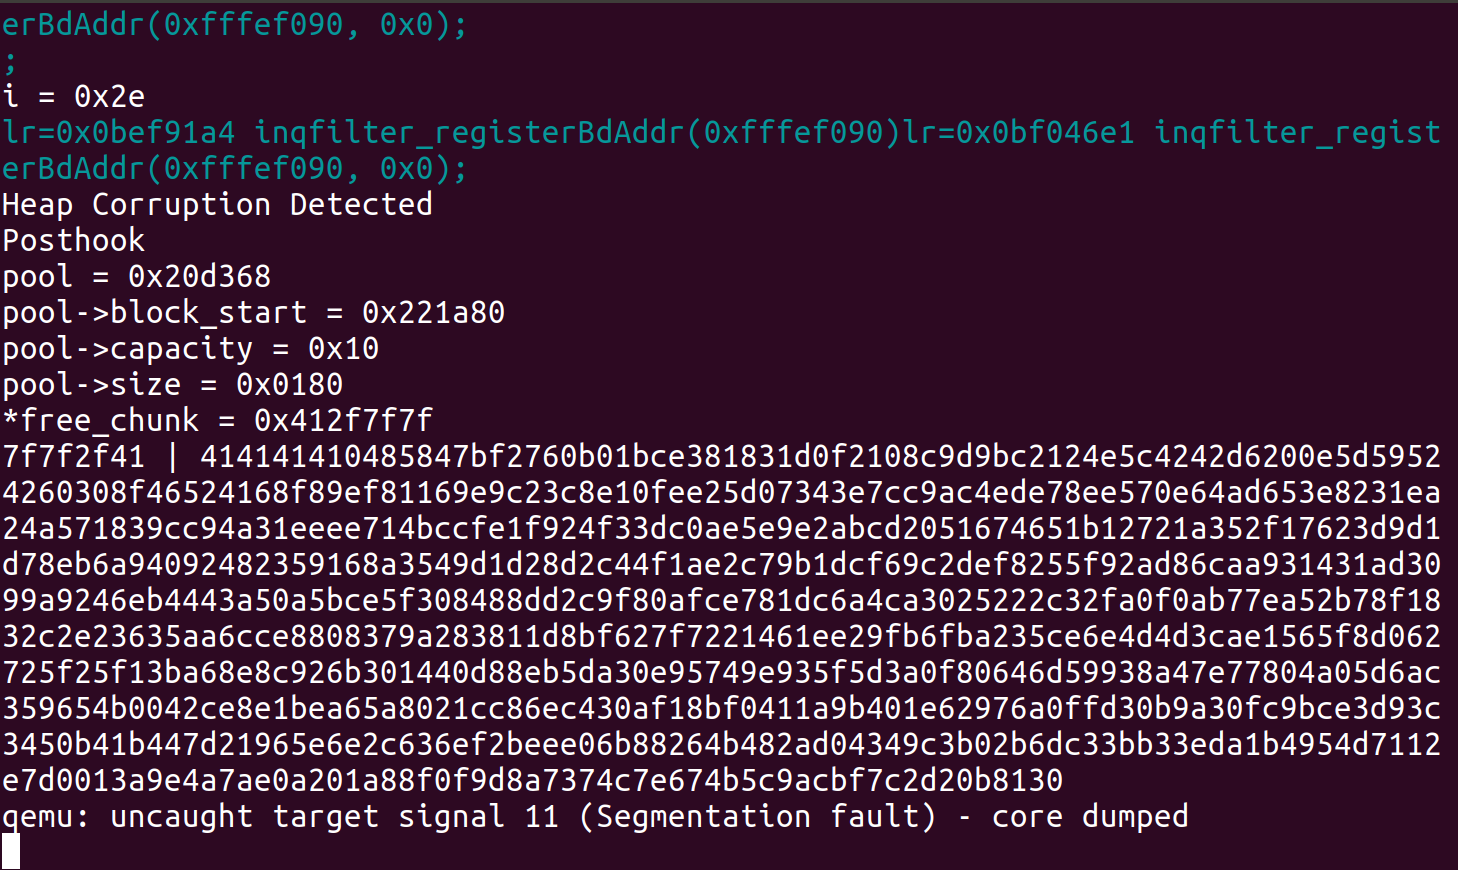
\includegraphics[width=\textwidth]{images/InqFilter.png}
    \caption{Emulating inqfilter.exe}
    \label{fig:inqfilter}
\end{figure}

\subsection{Reproducing CVE-2019-11916}
When a bluetooth device is trying to connect to a Bluetooth Low Energey(BLE) device or exchanging packets with a BLE device, This bug might trigger. So the problem is when the other BLE device sends a packet which has a PDU more than 252 bytes. In the receiving firmware side, it causes a heap corruption error. 

In my experiment, I tried to connect to a BLE device with the virtual bluetooth device. While fuzzer is feeding the virtual bluetooth device with random BLE packets. At a point a packet with packet length \verb|oxff| caused the crash. Figure \ref{fig:ble_cve} shows the experiemnt. In the right side our virtual bluetooth device is trying to connect a ble device with the command \verb|lecc|. Left side shows what is happening inside it's firmware. 
\begin{figure}[!h]
    \centering
    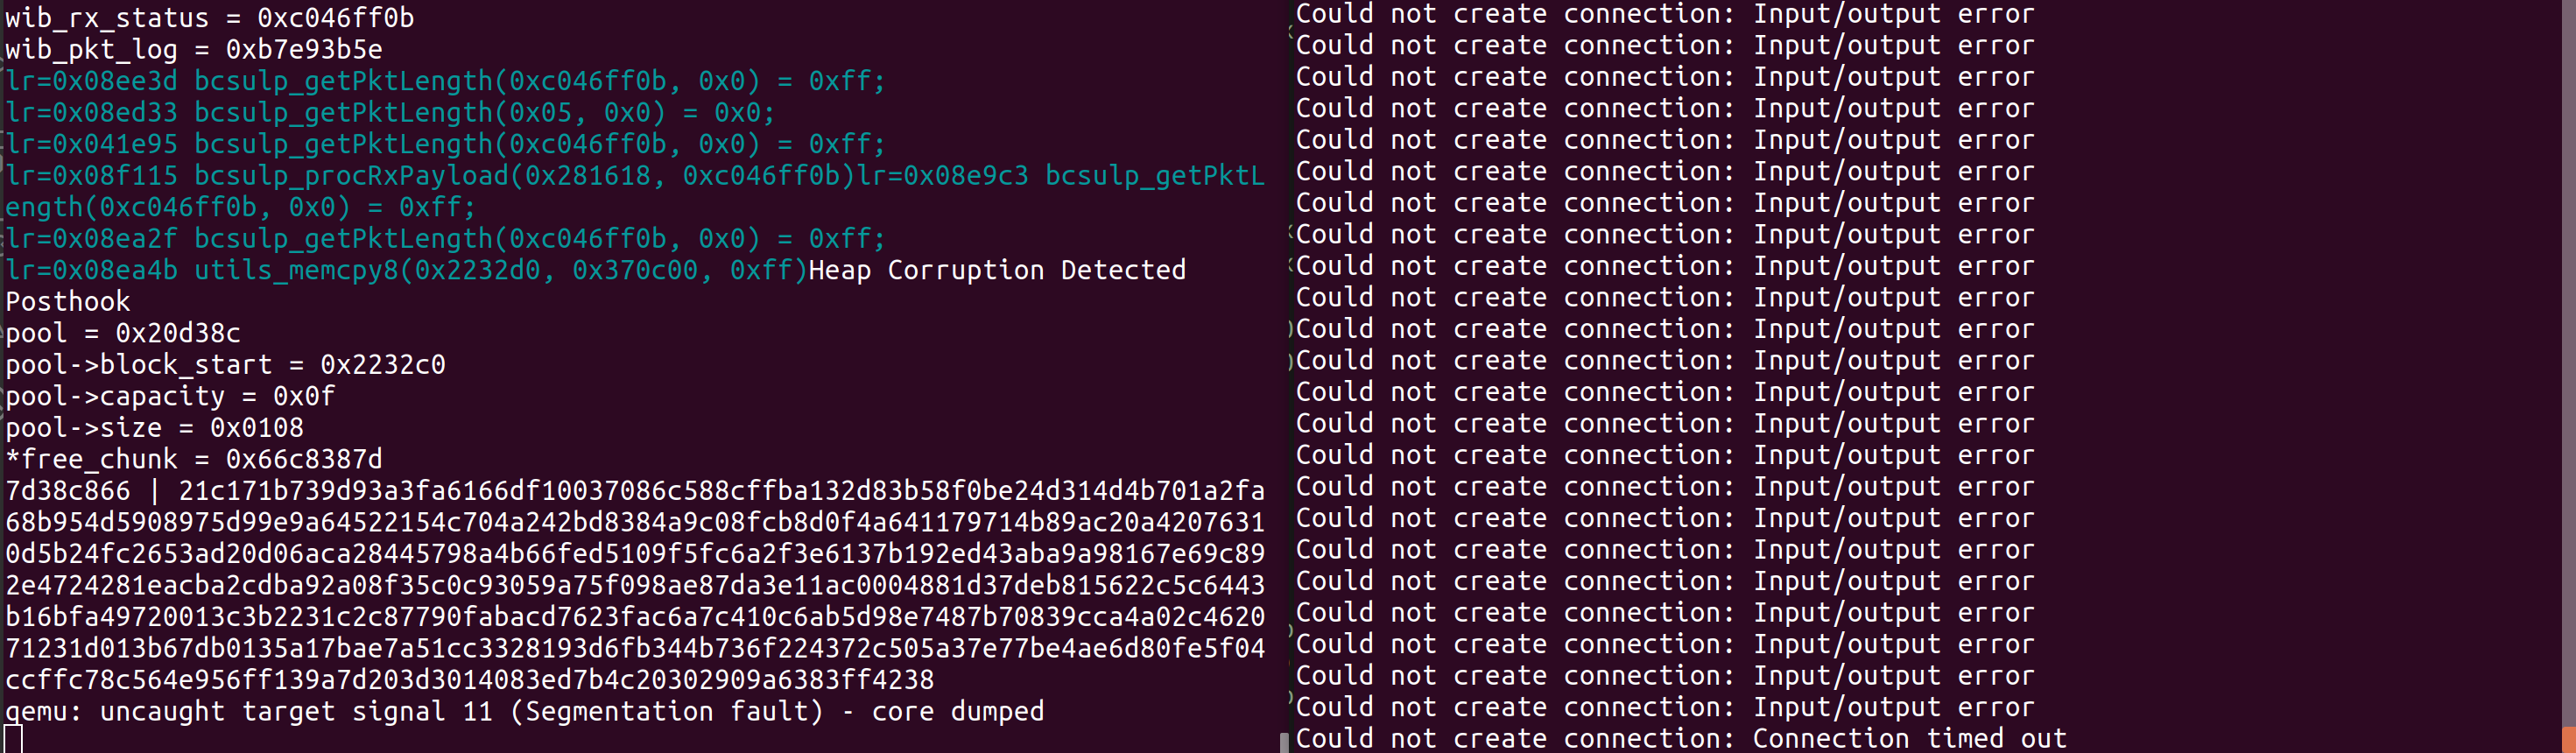
\includegraphics[width=\textwidth]{images/Second-cve.png}      \caption{Reproducing CVE-2019-11916}
    \label{fig:ble_cve}
\end{figure}

\section{Discussion}
As per deliverable mentioned above \ref{sec:deliverable}, I completed all the experiment I mentioned in the proposal. I also checked one more emulation \verb|hci_oracle.exe| which I didn't mention in the proposal. Due to time limit and device limitation I couldn't complete all the experiment mentioned in the article. But I would say I completed most part (6 emulations out of 8 and reproducing 2 CVEs) from the article. Focus of this article was about emulating a firmware to complete wireless fuzzing. I would focus was achieved completely.

% \begin{figure}[!h]
%     \centering
%     \begin{minipage}[b]{0.5\textwidth}
%         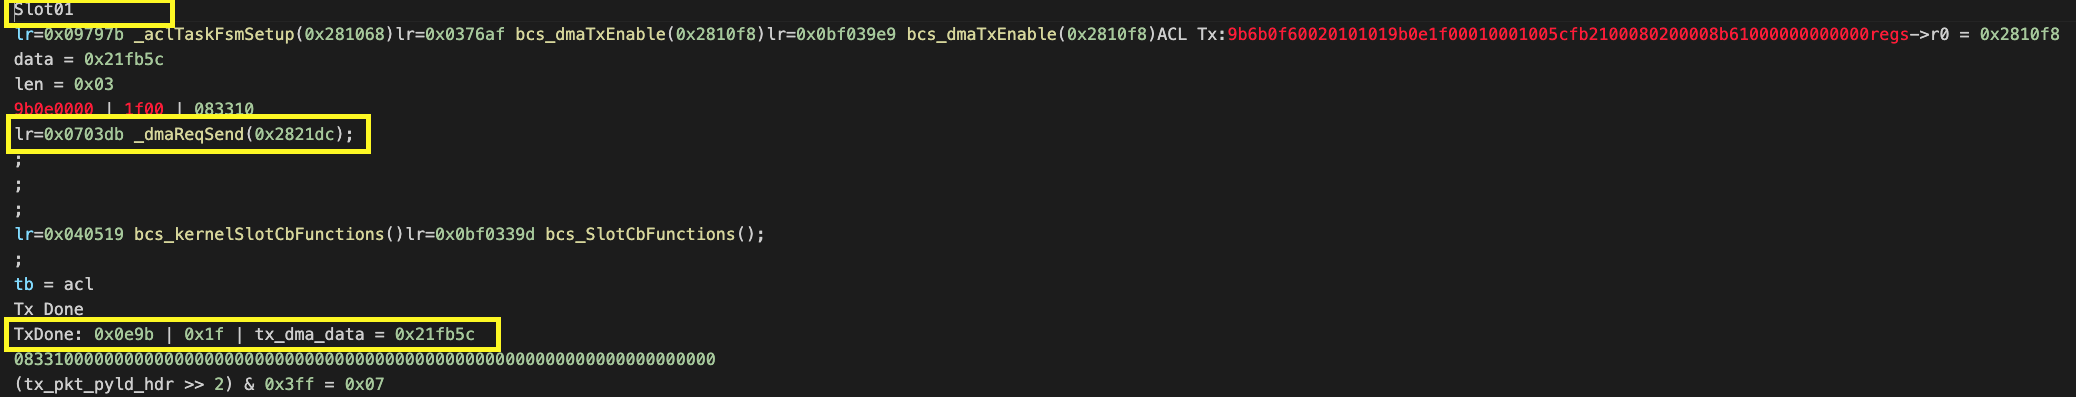
\includegraphics[width=\textwidth]{images/acl_Send_data.png}
%         \caption{ACL packet sending}
%     \end{minipage}
%   \hfill
%   \begin{minipage}[b]{0.4\textwidth}
%     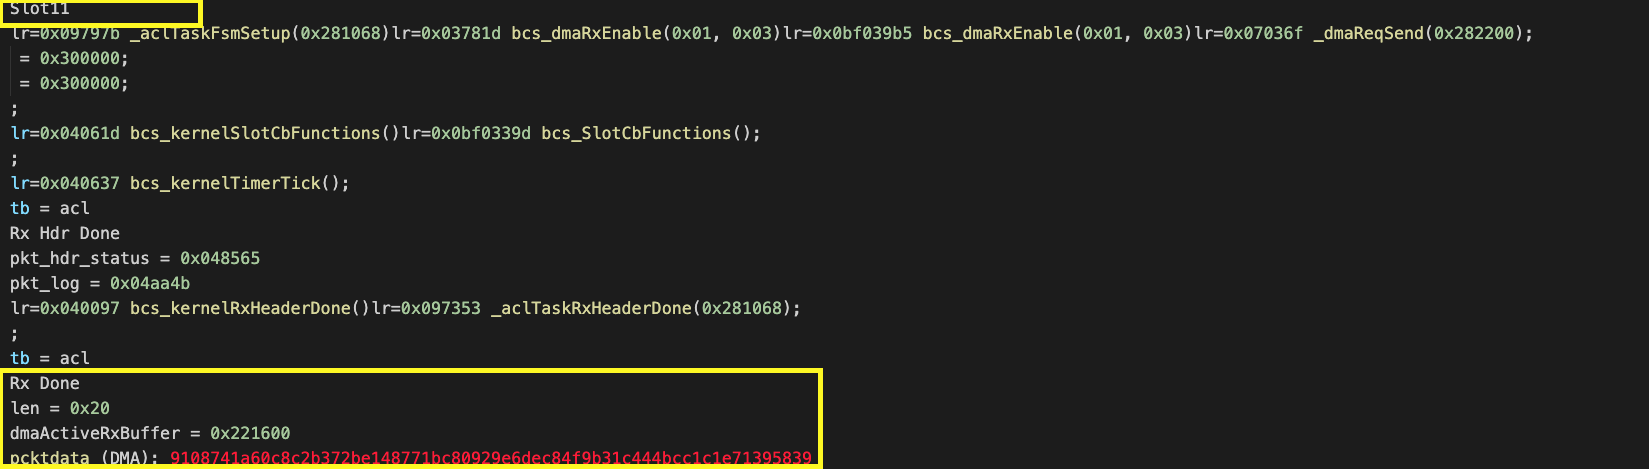
\includegraphics[width=\textwidth]{images/acl_receive_data.png}
%     \caption{ACL packet receiving}
%   \end{minipage}
% \end{figure}

\printbibliography

\end{document}
